\documentclass{article}
\usepackage[margin=1.0in]{geometry}
\usepackage{polski}
\usepackage[utf8]{inputenc}
\date\today
\usepackage{amssymb, amsthm, amsmath}
\usepackage{graphicx}

\usepackage{subcaption}

\title{HPC - MPI}
\author{Tomasz Kępa \\ \texttt{tk359746@students.mimuw.edu.pl}}

%%%% My macros
\newcommand{\todo}[1]{\colorbox{yellow}{ \color{red} \textbf{TODO}: {#1}}}

\begin{document}
\maketitle


\section{Struktura plików}
Rozwiązanie podzielone jest na pliki w następujący sposób:
\begin{itemize}
  \item Struktury danych:
    \begin{itemize}
       \item \emph{config.h} -- struktura przechowująca sparsowane flagi przekazane do programu
       \item \emph{mpigroup.h} -- struktura definiująca grupę obliczeniową (wszystkie procesy, grupy replikacyjne, warstwy)
       \item \emph{matrix.h matrix.cpp} -- struktury przechowujące informacje o macierzy oraz macierze rzadkie i gęste
    \end{itemize}
  \item \emph{densematgen.h densematgen.cpp} -- pliki dostarczone razem z treścią zadania służacego do generowania macierzy gęstej
  \item \emph{utils.h} -- mniej istotne pomocnicze funkcje
  \item \emph{matrixmul.h matrixmul.cpp} -- definicje głównych etapów obliczeń i główny program, implementacje w następujących plikach:
    \begin{itemize}
      \item \emph{initialization.cpp} -- wczytywanie macierzy A, generowanie macierzy B, początkowa dystrybucja danych (jak dla $c=1$)
      \item \emph{replication.cpp} -- rozsyłanie danych między procesami z tych samych grup replikacyjnych, w przypadku algorytmu InnerABC
                                                         dodatkowo wykonanie początkowego przesunięcia fragmentów macierzy A
      \item \emph{communication.cpp} -- operacja shift-and-compute (jeden krok obliczeń jednego procesu)
      \item \emph{multiplication.cpp} -- mnożenie macierzy i komunikacja z tym związana
      \item \emph{gathering.cpp} -- zbieranie wyników
    \end{itemize}
\end{itemize}

\section{Struktury danych}

Przed rozpoczęciem obliczeń wszystkie macierze są wyrównywane zerami, tak aby ilość wierszy i kolumn była podzielna przez ilość procesów.

\subsection{Metadane macierzy}
Najważniejsze informacje o macierzy przechowywane są w strukturze \emph{MatrixInfo}. Zawiera ona wszystkie informacje potrzebne 
do zaalokowania odpowiedniej ilości pamięci przed odbiorem nieznanej macierzy i z tego powodu wysyłana jest zawsze przez wysłaniem 
macierzy.

\subsection{Macierze rzadkie}
Macierze rzadkie przechowywane są w strukturze \emph{SparseMatrix}. Jest to dokładnie taki sam format jak format na wejściu, 
czyli CSR z trzema tablicami.
Taki format został wybrany z kilku powodów:
\begin{itemize}
  \item Nie trzeba tracić czasu na zmianę formatu podczas inicjalizacji
  \item Biblioteka MKL potrafi używać ten format (w wersji z czterema tablicami, ale przejście do tego fomatu nic nie kosztuje)
  \item Jest to format row-major, co jest korzystne dla ręcznej implementacji mnożenia macierzy
\end{itemize}

\subsection{Macierze gęste}
Macierze gęste przechowywane są w pojedynczej tablicy rozmiaru $rows \times cols$ w kolejności column-major.
Taki formata został wybrany z następujących powodów:
\begin{itemize}
  \item Jest to korzystna kolejność dla implemetacji lokalnego mnożenia macierz
  \item Procesy trzymają w swoich fragmentach całe kolumny oryginalnych macierzy, więc rozsyłanie i zbieranie macierzy jest dużo prostsze
           w takim formacie i nie wymaga wykonywania dodatkowych kopii (lokalnych) macierzy
\end{itemize} 

\section{Intesywność numeryczna}
Oznaczenia:
\begin{itemize}
  \item $d$ -- oznaczmy średnią ilość niezerowych elementów w jednym wierszu macierzy A
  \item $e$ -- ilość mnożeń macierzy A przez macierz B
  \item $n$ -- wymiary macierzy A, B i C
\end{itemize}

\subsection{Operacje zmiennoprzecinkowe}
Do policzenia jednej komórki macierzy C trzeba wykonać średnio $d$ mnożeń i $d-1$ dodawań
w jednym kroku.
Zatem do policzenia macierzy C potrzebne jest $(2d-1) \cdot n^2 \cdot e$ operacji zmiennoprzecinkowych.

\subsection{Transfery pamięci}
Rozpatrzmy to podobnie jak poprzednio. W tym przypadku istotne staje się jak trzymana jest macierz rzadka A.
Założę teraz, że jest to format CRS.
W jednym kroku, do policzenia jednej komórki potrzebujemy odczytać jeden wiersz macierzy A i jedną kolumnę macierzy B.
Jeśli chodzi o zapisy to potrzebujemy to zrobić to tylko raz w macierzy C.

Wczytanie wiersza macierzy A wymaga odczytania średnio $(4 \cdot 2 + 4 \cdot d + 8 \cdot d$ bajtów ($2$ el. tablicy trzymającej długości wierszy,
$d$ indeksów kolumn, $d$ elementów macierzy A). W macierzy B czytamy średnio $8 \cdot d$ bajtów (d elementów).
Na koniec jeszcze musimy wykonać jeden zapis w macierzy $C$

Razem daje to $16 + 20d$ bajtów na element macierzy C w jednym kroku.

W sumie policzenie całej macierzy C wymaga transferu $(16 + 20d) \cdot n^2 \cdot e$ bajtów.


\section{Komunikacja}
W obu algorytmach (o ile $c \neq 1$) procesy podzielone są w dwuwymiarową siatkę. Najpierw, wszystkie procesy podzielone są w grupy
replikacyjne rozmiaru $c$, a pomiędzy tymi grupami, procesy o tych samych rangach wyznaczają warstwy. Warstw musi być oczywiście $c$.

W trakcie inicjalizacji koordynator wczytuje macierz A i wysyła odpowiednie fragmenty do wszystkich procesów.
Następnie, procesy w tych samych grupach replikacji wymieniają między sobą swoje fragmenty macierzy A (i C dla InnerABC).
W trakcie obliczeń procesy wysyłają komunikaty tylko wewnątrz swojej warstwy.
W trakcie końcowego zbierania danych komunikacja wygląda inaczej w obu algorytmach i szerzej opisana jest
w części poświęconej optymalizacjom.

\section{Optymalizacje}
\subsection{MPI}
Przy implementacji największy nacisk położyłem na efektywne wykorzystanie możliwości danych przez MPI:
\begin{itemize}
\item Większość komunikacji jest asynchroniczna i przepleciona z obliczeniami. 
\item Początkowe rozsyłanie macierzy przez koordynatora odbywa się tabela po tabeli. 
         Po wysłaniu jednej tabeli mechanizmem \emph{scatter} (asynchronicznie), 
         koorydator od razu zabiera się za przygotowanie kolejnej.
\item Przesyłanie macierzy w trakcie replikacji w grupie replikacyjnej 
         odbywa się przez customowe komunikatory za pomocą mechanizmu \emph{broadcast}.
\item Przesyłanie macierzy wewnątrz warstw (\emph{shift}) w trakcie obliczeń przeplecione jest z lokalnie wykonywanym mnożeniem.
\item Zbieranie macierzy C wewnątrz grupy replikacyjnej odbywa się za pomocą mechanizmu \emph{reduce} (tylko w InnerABC),
         operacja sumy. Zbieranie macierzy C w warstwie zerowe to zwykłe \emph{gather}.
\item Zliczanie liczby elementów większych od danego -- w przypadku ColumnA jest to zwykłe \emph{reduce} po wszystkich procesach,
         w przypadku InnerABC macierz C najpierw zbierana jest do warstwy 0 i dopiero w tej warstwie jest wykonywana redukcja
\end{itemize}

Macierz A dzielona jest między procesy po równej ilości kolumn/wierszy. Innych opcji nie rozważałem ponieważ dokładnie tak
to było opisane w artykule opisującym algorytmy.

\subsection{Flagi kompilacji}
Najlepsze wyniki uzyskałem na kompilatorze \textbf{Cray}. Włączyłem następujące opcje:
\begin{itemize}
  \item \emph{-O3} -- domyślne optymalizacje
  \item \emph{-hfp3} -- optymalizacje operacji zmiennoprzecinkowych
  \item \emph{-h vector3} -- wektoryzacja operacji wykonywanych w pętlach
  \item \emph{-hipa4 -hwp -h pl=...} -- automatyczne inline'owanie funkcji
\end{itemize}

\subsection{Lokalne mnożenie}
Formaty macierzy zostały dobrane tak, aby było jak najmniej skoków w tablicach reprezentujących macierze.
Zatem macierz A jest row-major, macierze B i C są column-major.

\subsection{OpenMP}
Wykonałem próbę użycia równoległej implementacji MKL (używającej OpenMP). Wyniki były znacznie gorsze niż przy
wykorzystaniu wersji sekwencyjnej i poleganiu na MPI, dlatego nie próbowałem używać OpenMP w mojej implementacji.

\section{Skalowalność}

\subsection{Silna skalowalność}

Testy silnej skalowalności zostały przeprowadzone na dwóch macierzach A. 
Pierwsza miała $n=50000$ wierszy i $d=1000$ wartości w każdym wierszu. Druga -- $n=100000, d=100$.
W pierwszy przypadku mnożenie było wykonywane $e=5$ razy, w drugim $e=2$.
W obu przypadkach czas wczytywania macierzy wynosił ok. $9.5s$
Wyniki zostały przedstawione na rys.~\ref{fig:scal_strong_1} i rys.~\ref{fig:scal_strong_2}.

\begin{figure}[ht!]
    \centering
    \begin{subfigure}[b]{0.45\textwidth}
        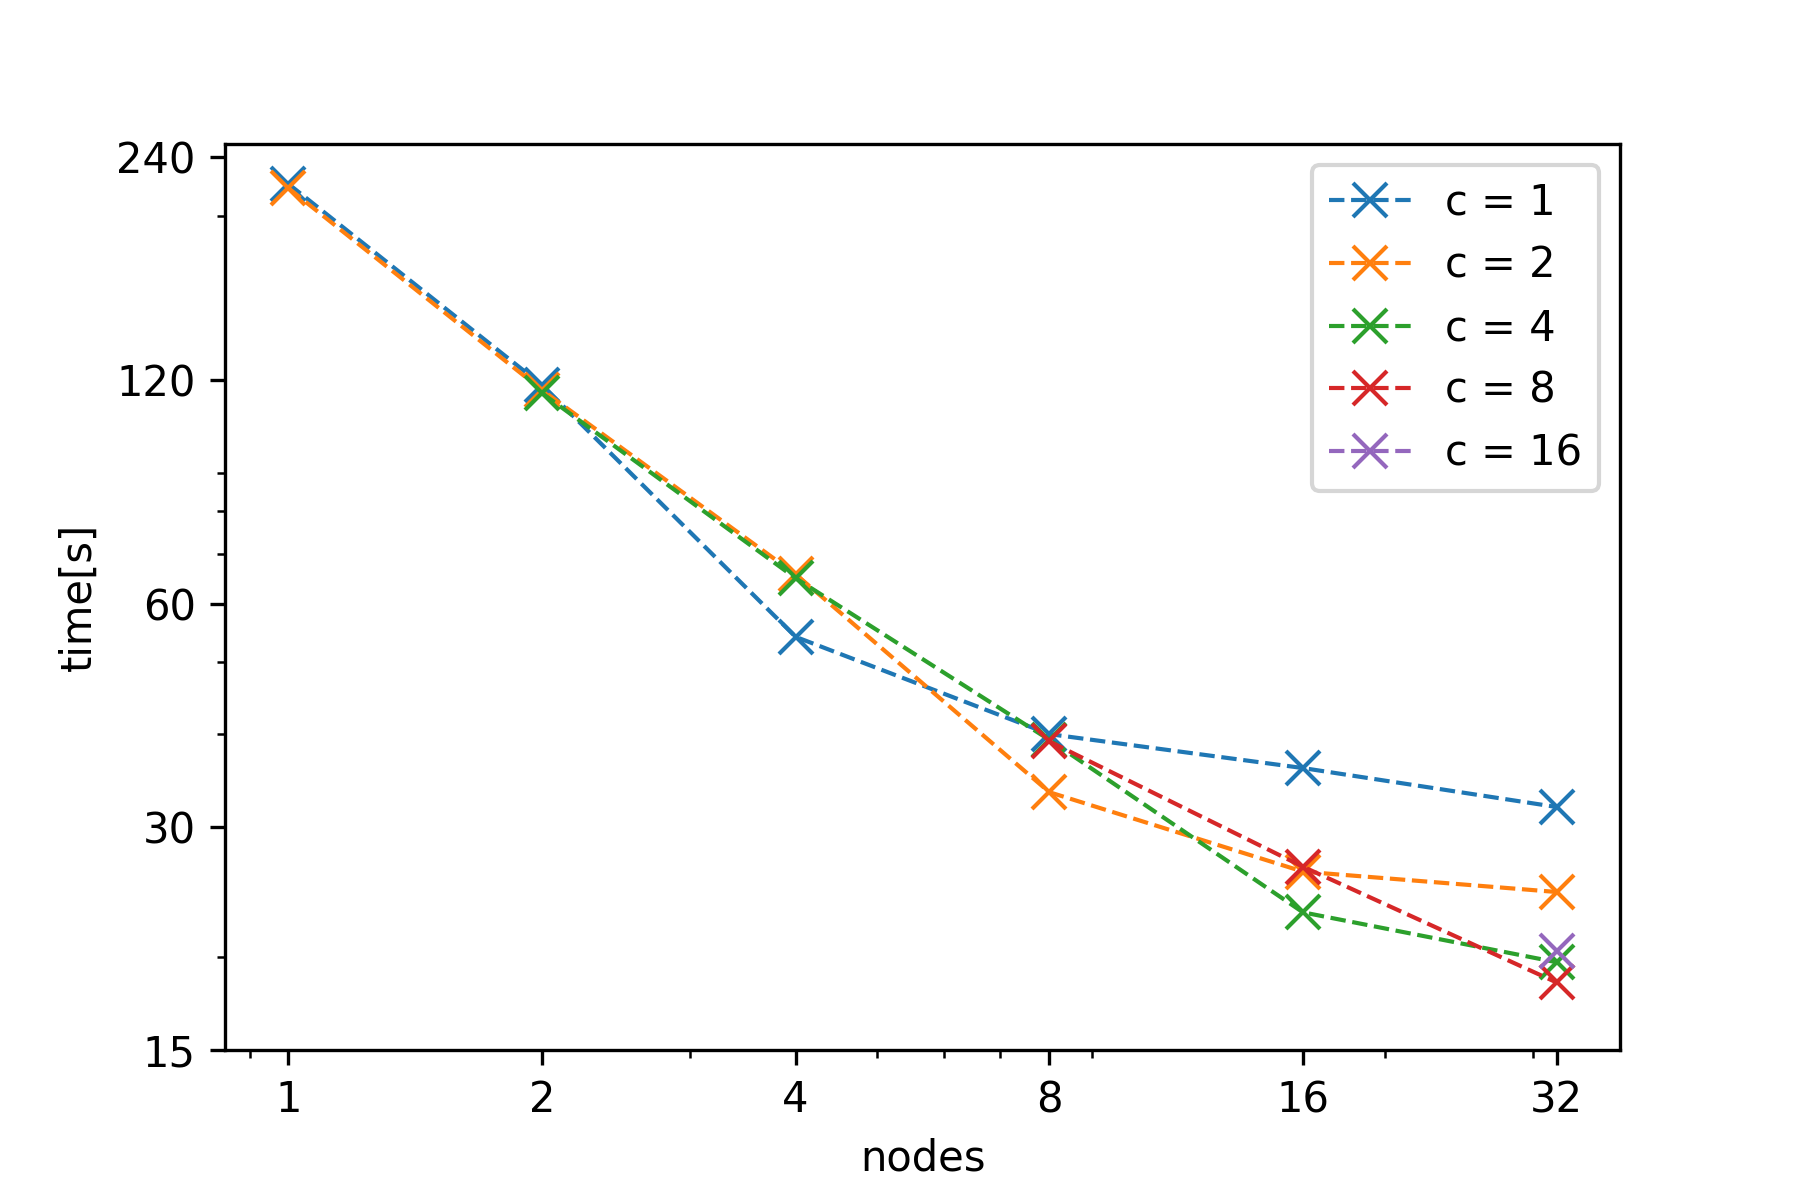
\includegraphics[width=\textwidth]{charts/s_50000_1000_5}
        \caption{ColumnA, no MKL}
    \end{subfigure}
    \begin{subfigure}[b]{0.45\textwidth}
        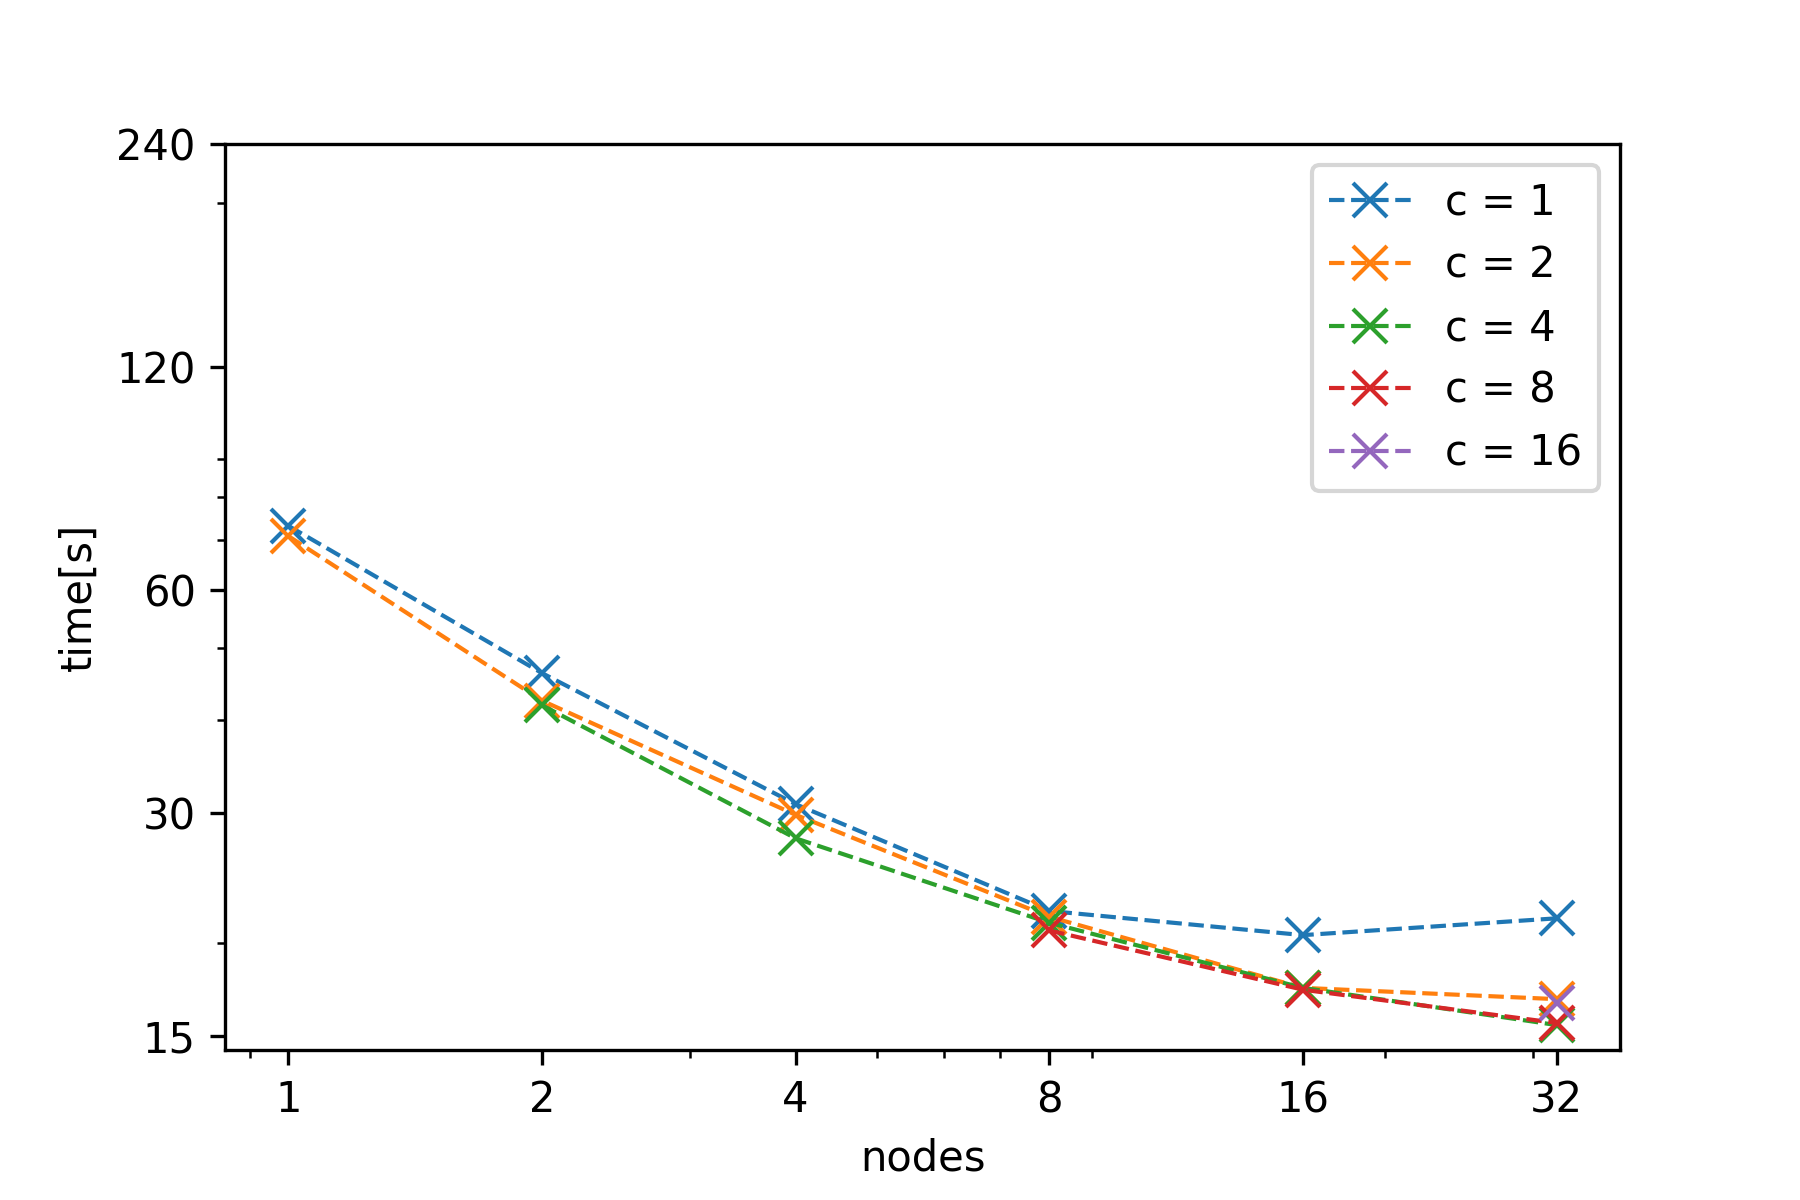
\includegraphics[width=\textwidth]{charts/s_50000_1000_5_m}
        \caption{ColumnA, MKL}
    \end{subfigure}
    \begin{subfigure}[b]{0.45\textwidth}
        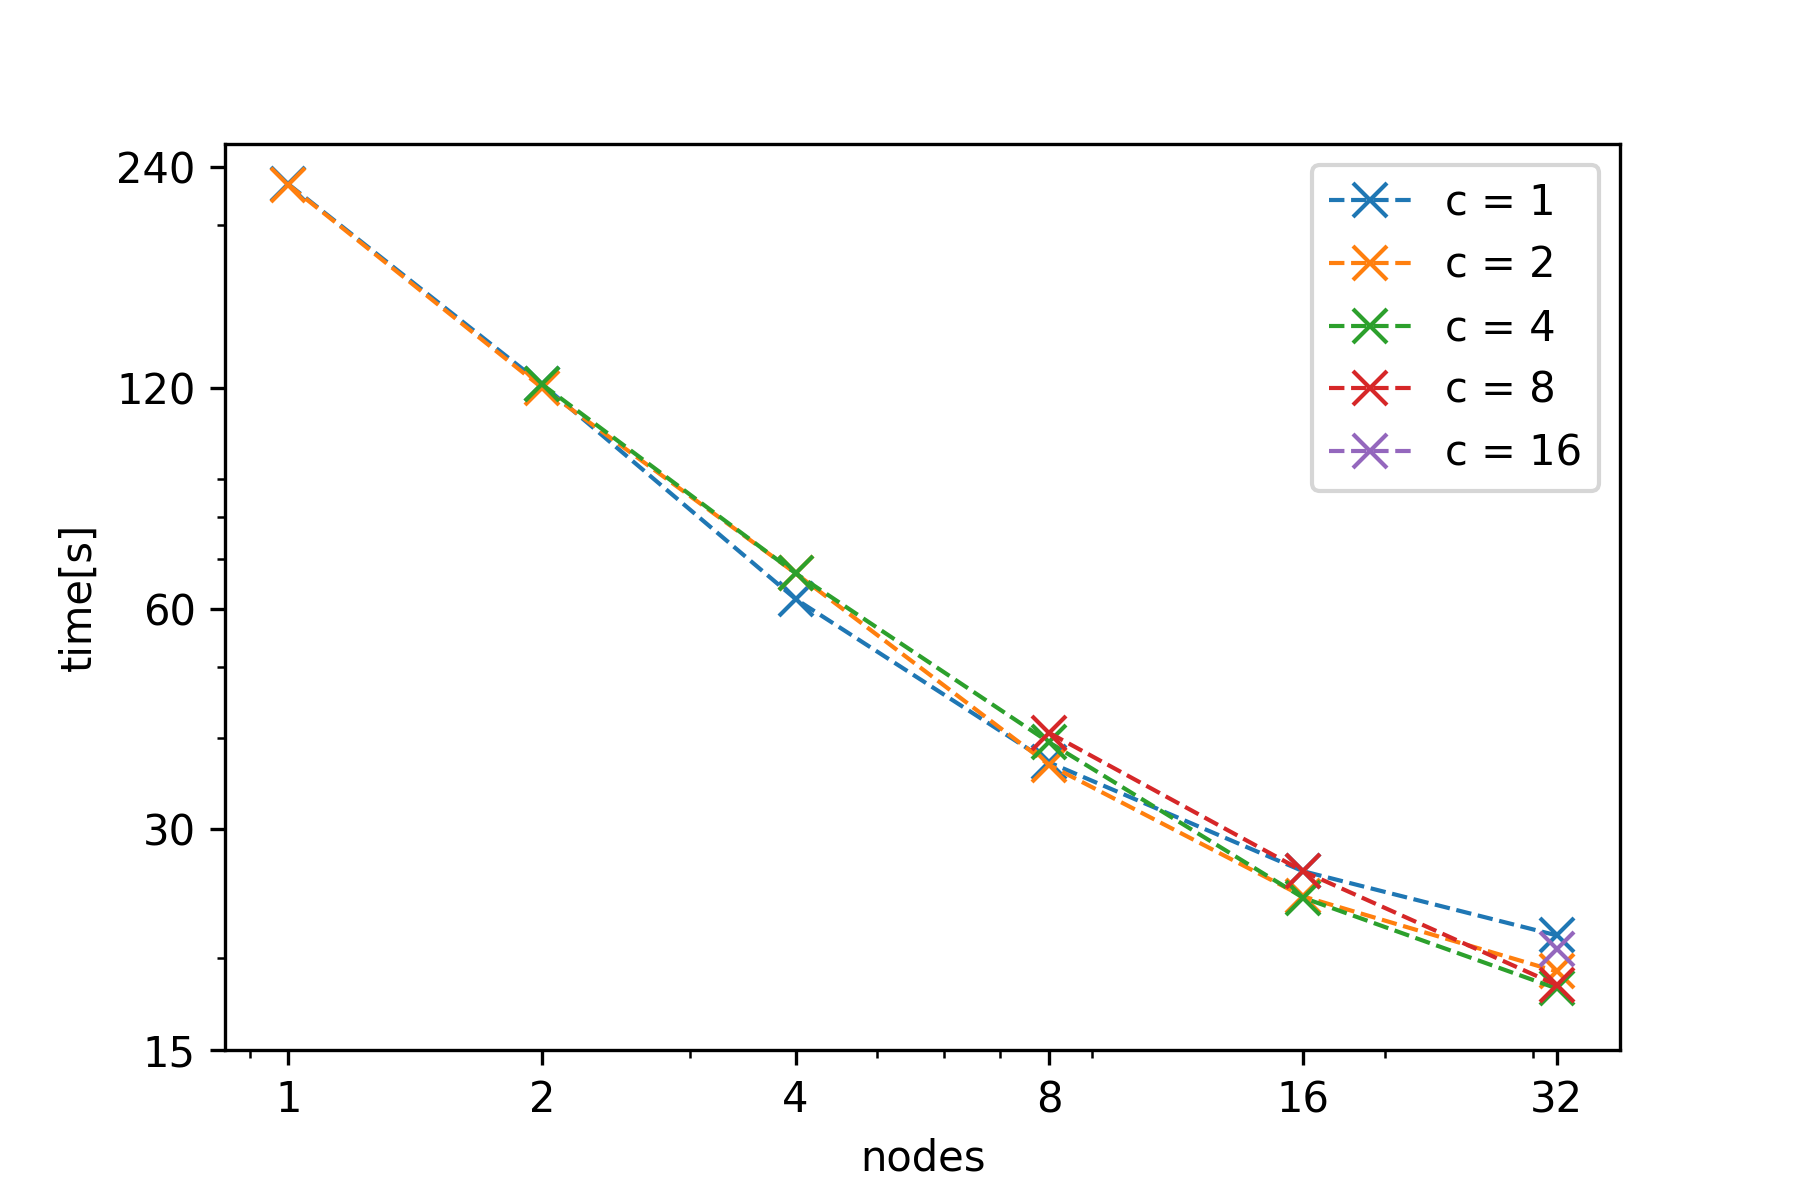
\includegraphics[width=\textwidth]{charts/s_50000_1000_5_i}
        \caption{InnerABC, no MKL}
    \end{subfigure}
    \begin{subfigure}[b]{0.45\textwidth}
        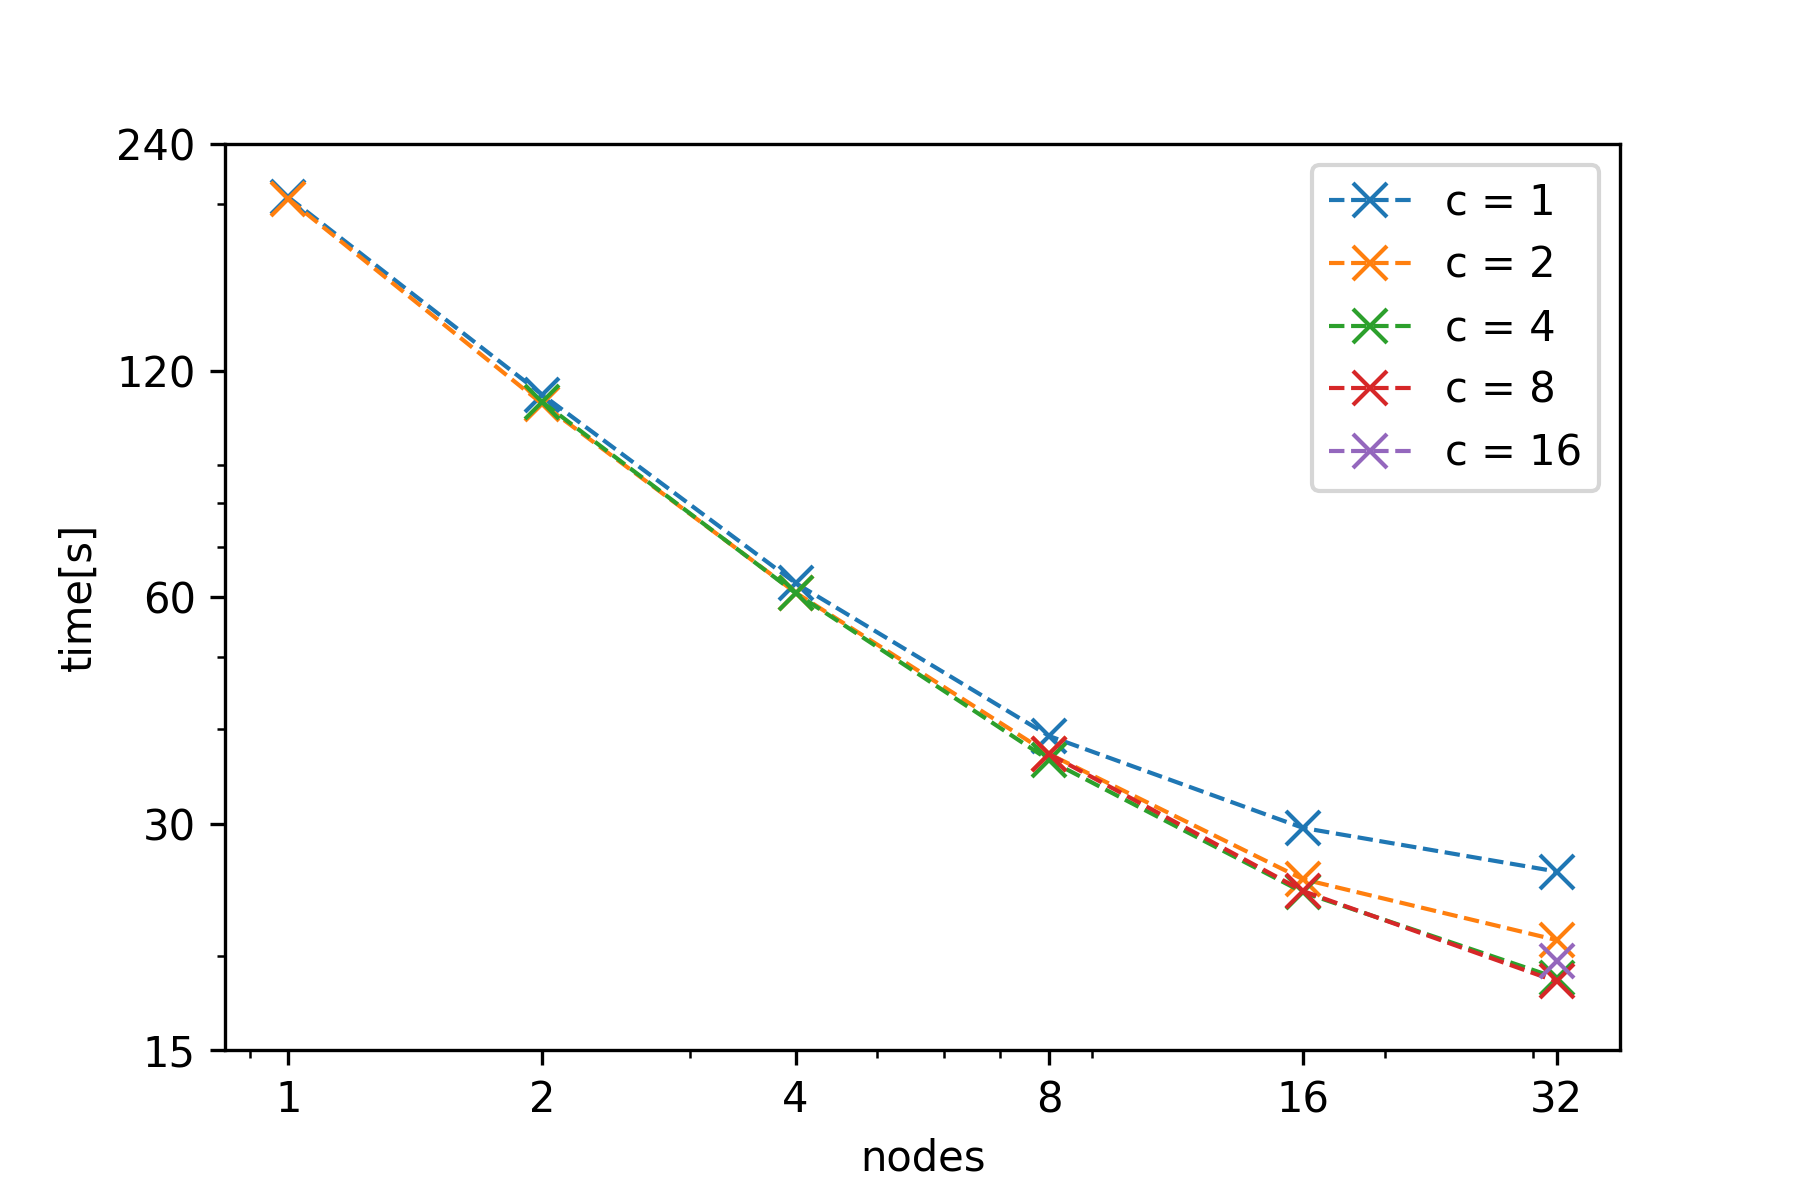
\includegraphics[width=\textwidth]{charts/s_50000_1000_5_i_m}
        \caption{InnerABC, MKL}
    \end{subfigure}
    \caption{Silna skalowalność. Czasy dla $n=50000, d=1000, e=5, \text{tasks-per-node}=24$}\label{fig:animals}
    \label{fig:scal_strong_1}
\end{figure}

\begin{figure}[ht!]
    \centering
    \begin{subfigure}[b]{0.45\textwidth}
        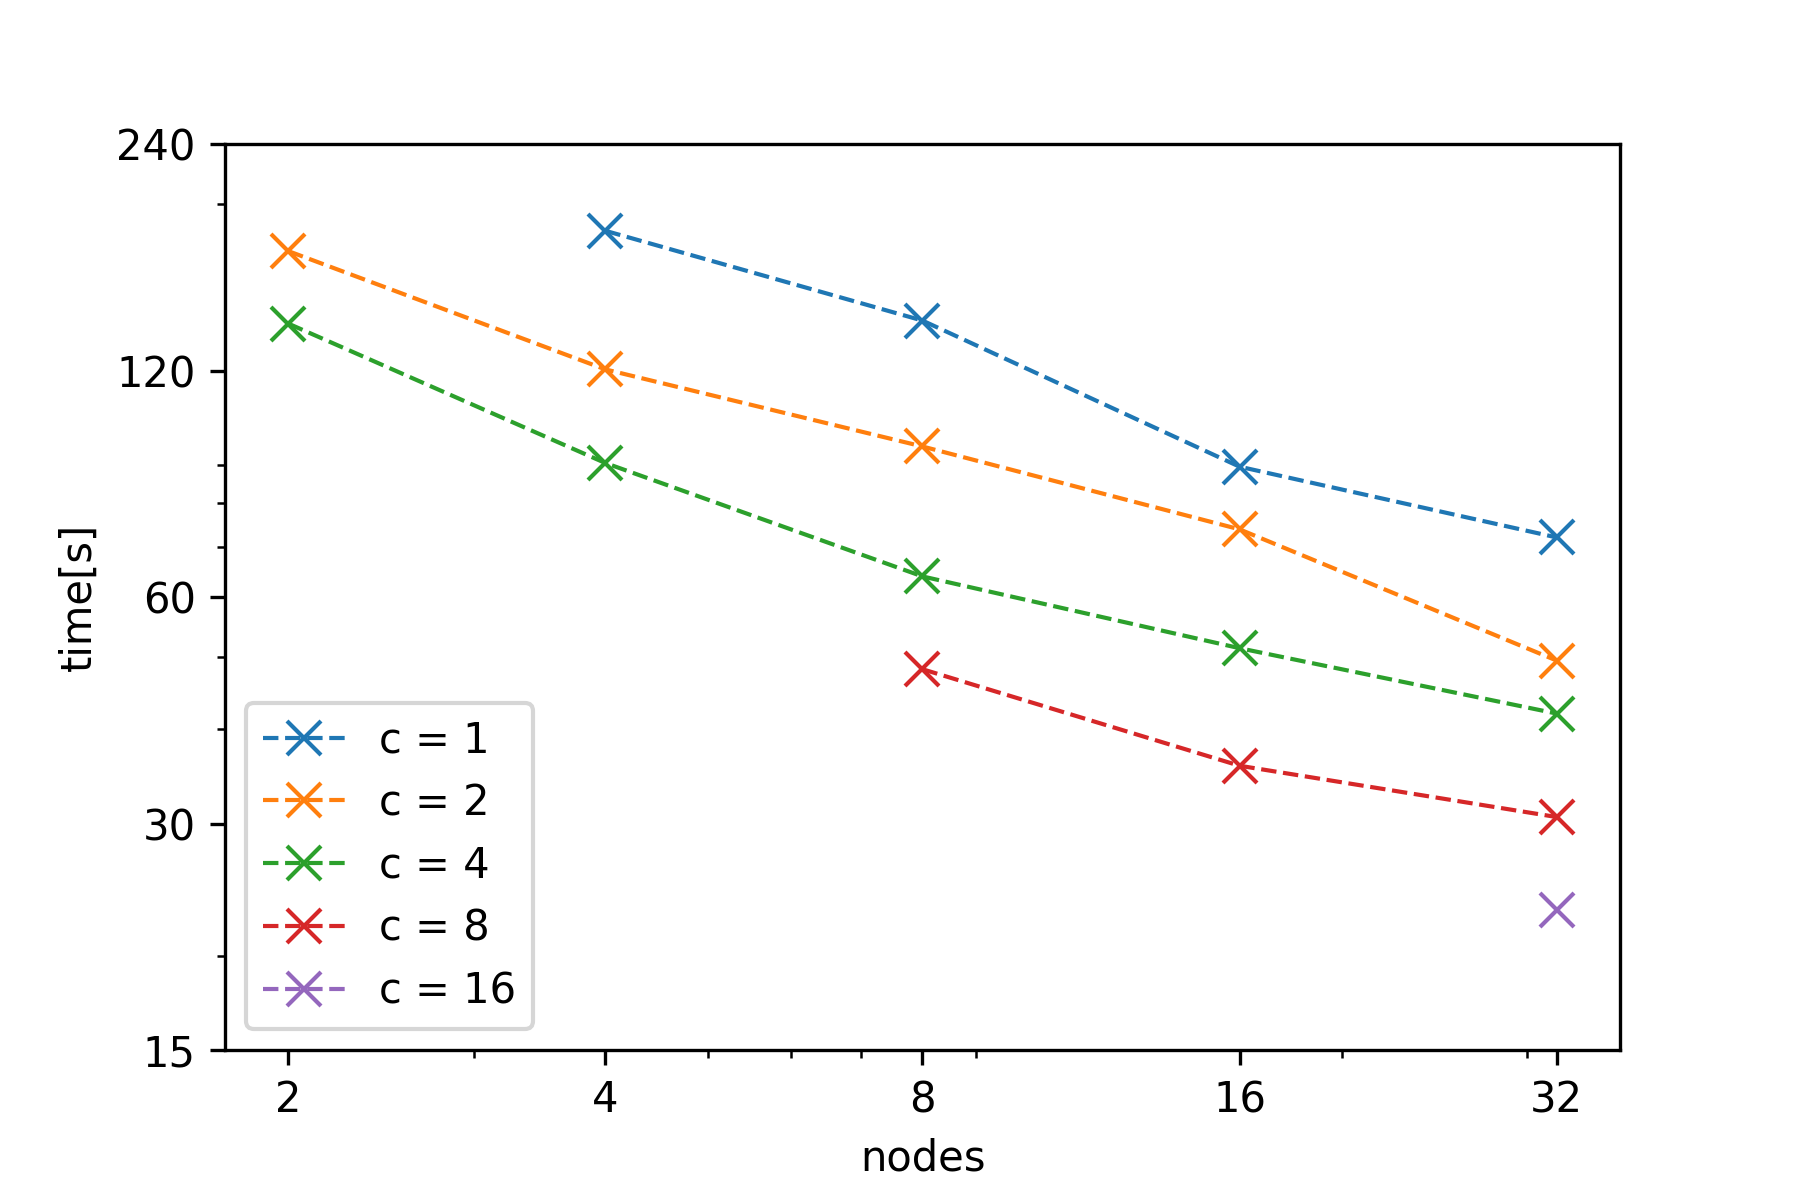
\includegraphics[width=\textwidth]{charts/s_100000_100_2}
        \caption{ColumnA, no MKL}
    \end{subfigure}
    \begin{subfigure}[b]{0.45\textwidth}
        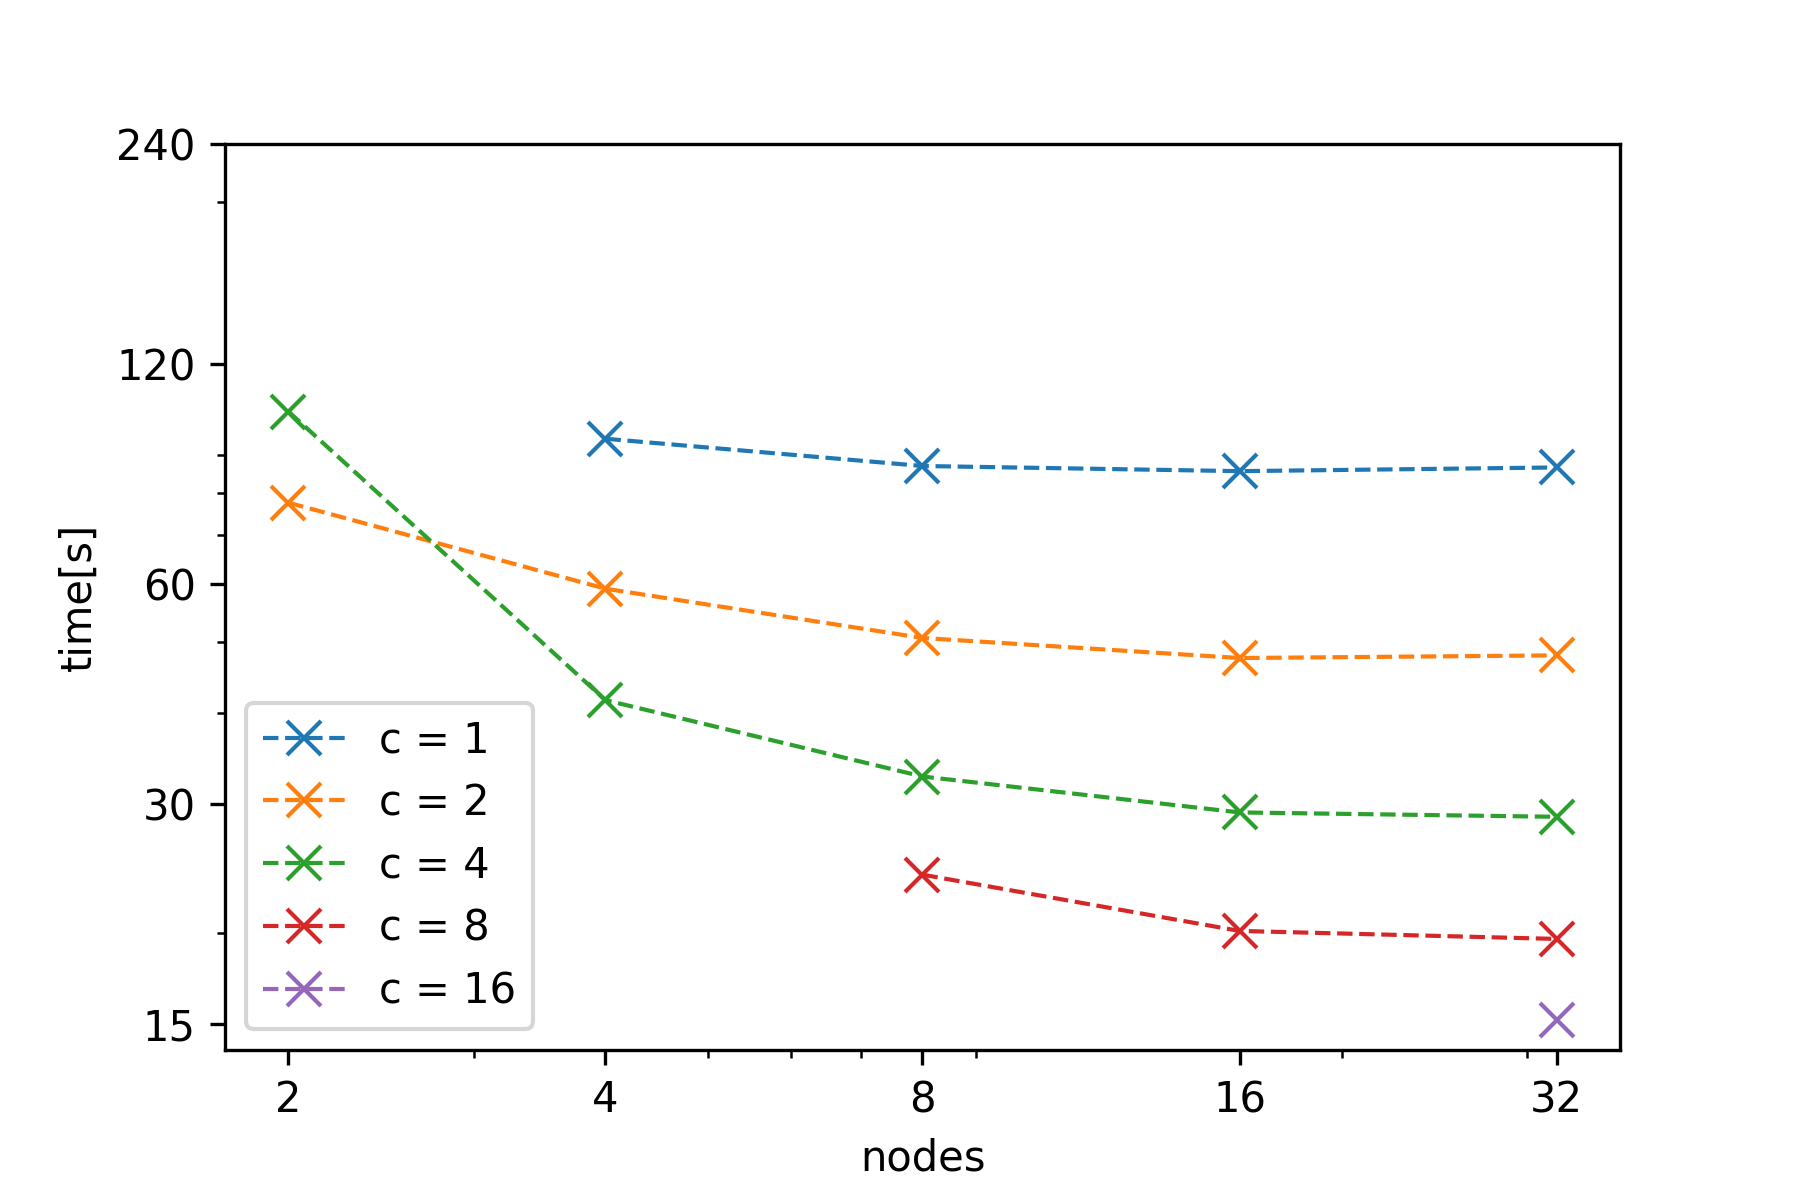
\includegraphics[width=\textwidth]{charts/s_100000_100_2_m}
        \caption{ColumnA, MKL}
    \end{subfigure}
    \begin{subfigure}[b]{0.45\textwidth}
        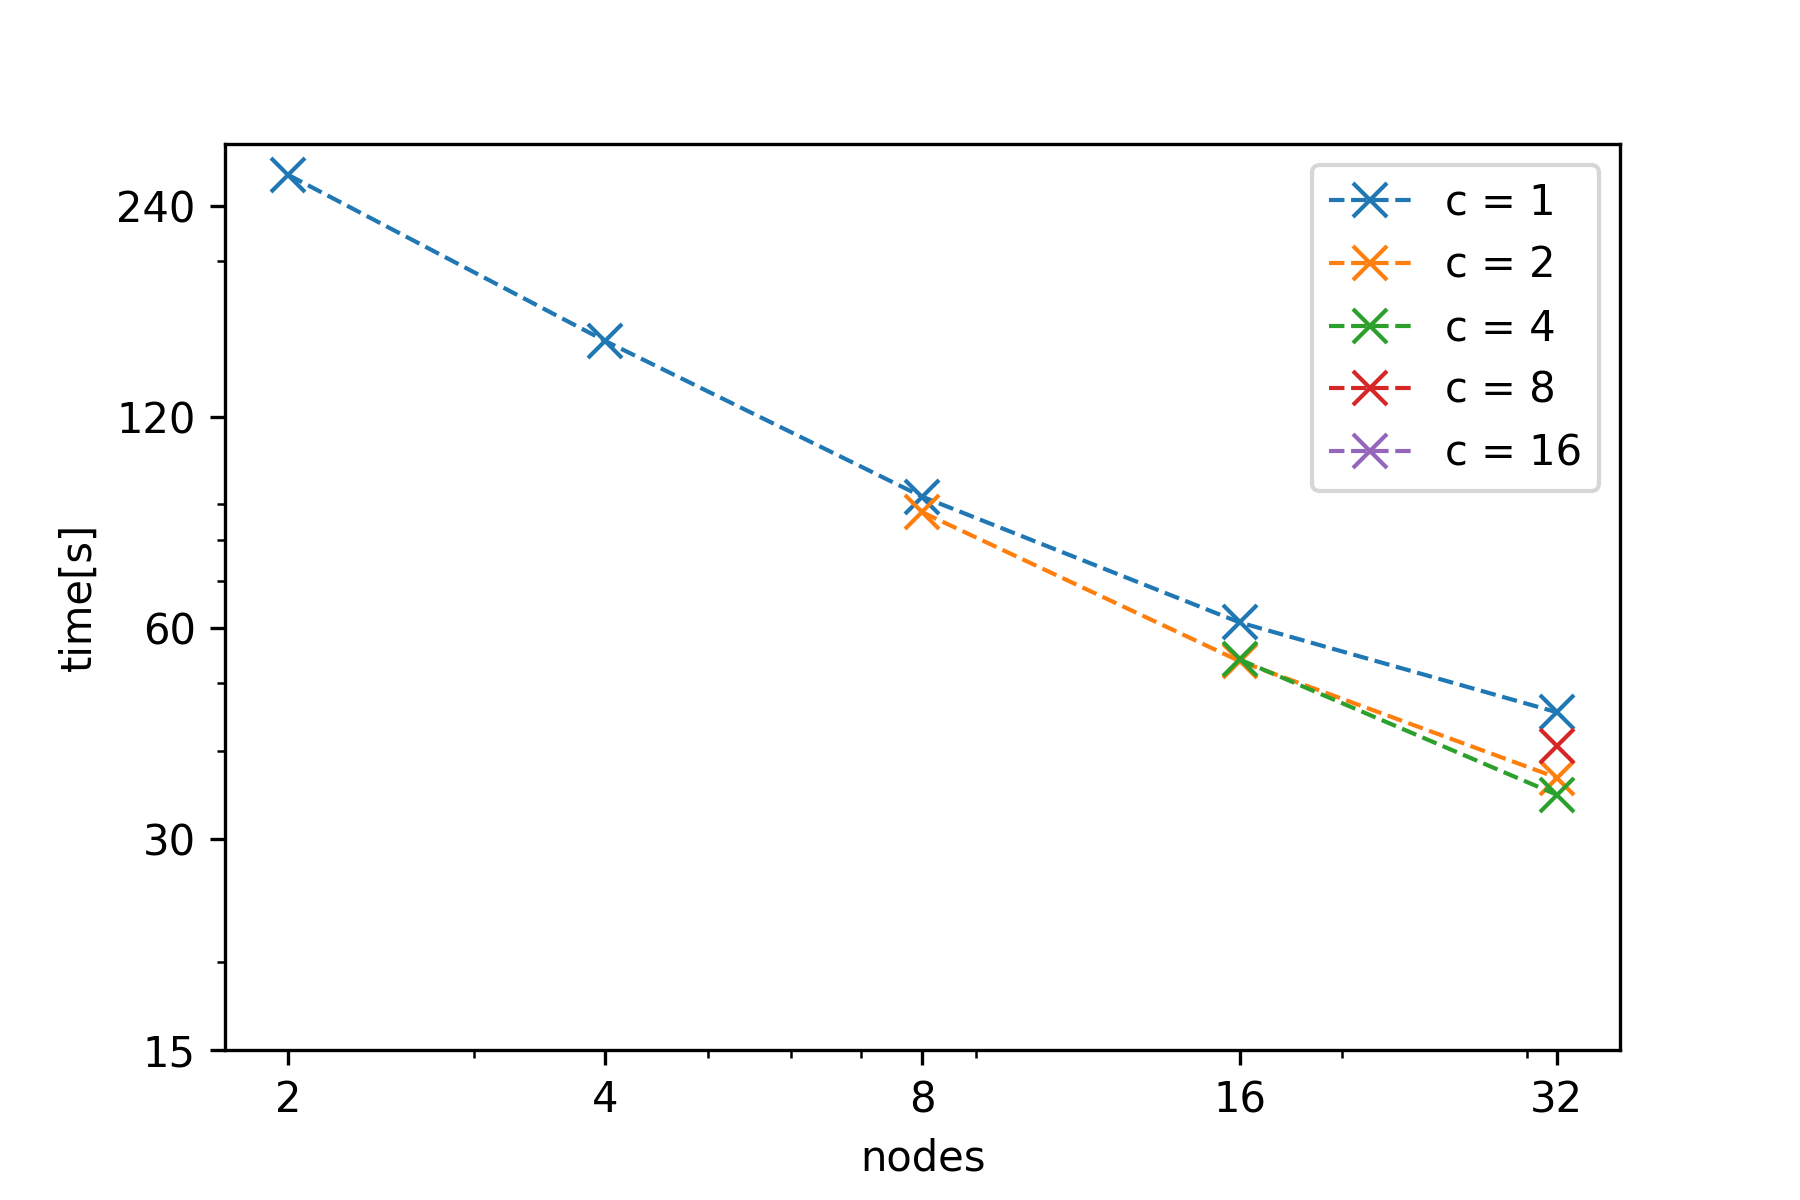
\includegraphics[width=\textwidth]{charts/s_100000_100_2_i}
        \caption{InnerABC, no MKL}
    \end{subfigure}
    \begin{subfigure}[b]{0.45\textwidth}
        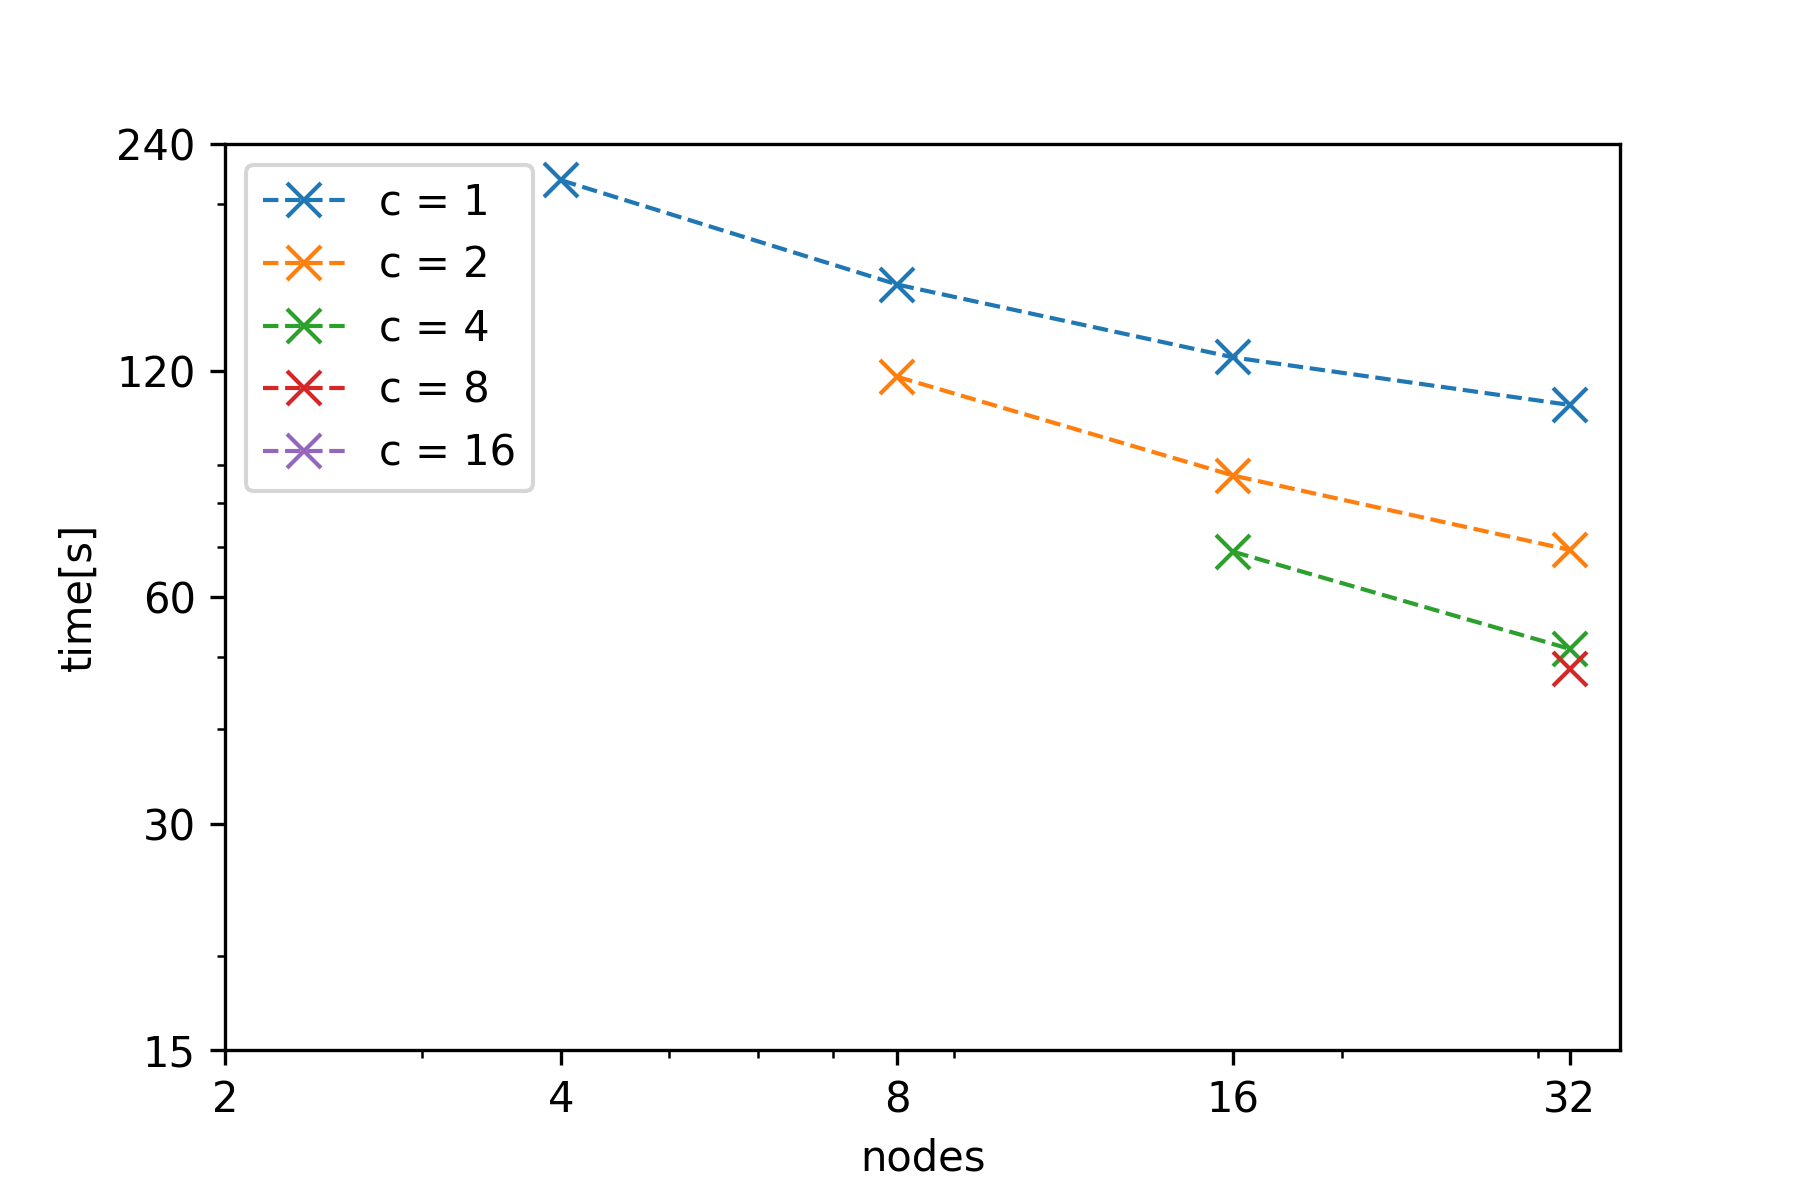
\includegraphics[width=\textwidth]{charts/s_100000_100_2_i_m}
        \caption{InnerABC, MKL}
    \end{subfigure}
    \caption{Silna skalowalność. Czasy dla $n=100000, d=100, e=2, \text{tasks-per-node}=24$}\label{fig:animals}
    \label{fig:scal_strong_2}
\end{figure}

\subsection{Słaba skalowalność}

Testy silnej skalowalności zostały przeprowadzone na macierzy $n=100000, d=100$.
Zmienna była liczba wykonywanych mnożesz i wynosiła $e = nodes \times 5$.
Parametr $c$ został ustalony na $c=2$
Czas wczytywania macierzy wynosił ok. $9.5s$
Wyniki zostały przedstawione na rys.~\ref{fig:scal_weak}.

\begin{figure}[ht!]
    \centering
    \begin{subfigure}[b]{0.45\textwidth}
        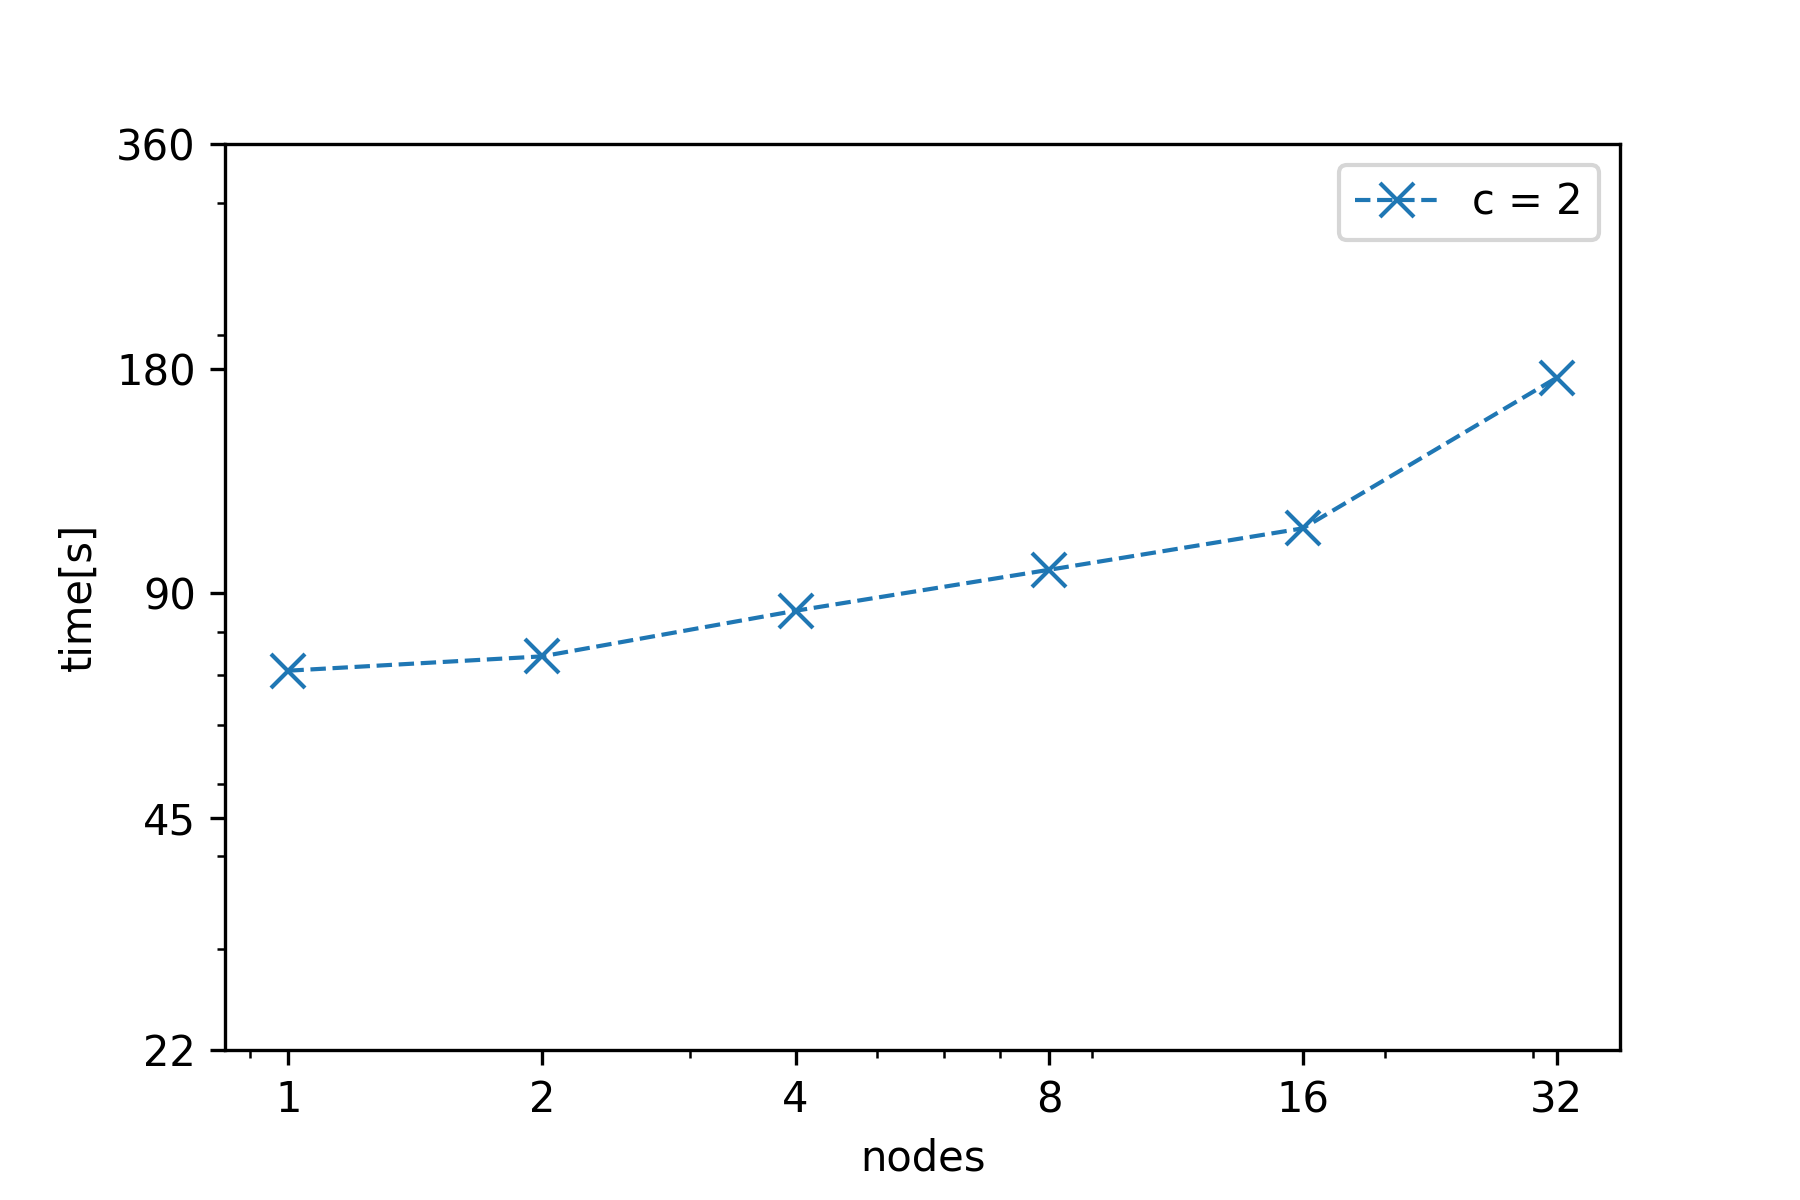
\includegraphics[width=\textwidth]{charts/s_50000_1000_weak_m}
        \caption{ColumnA, MKL}
    \end{subfigure}
    \begin{subfigure}[b]{0.45\textwidth}
        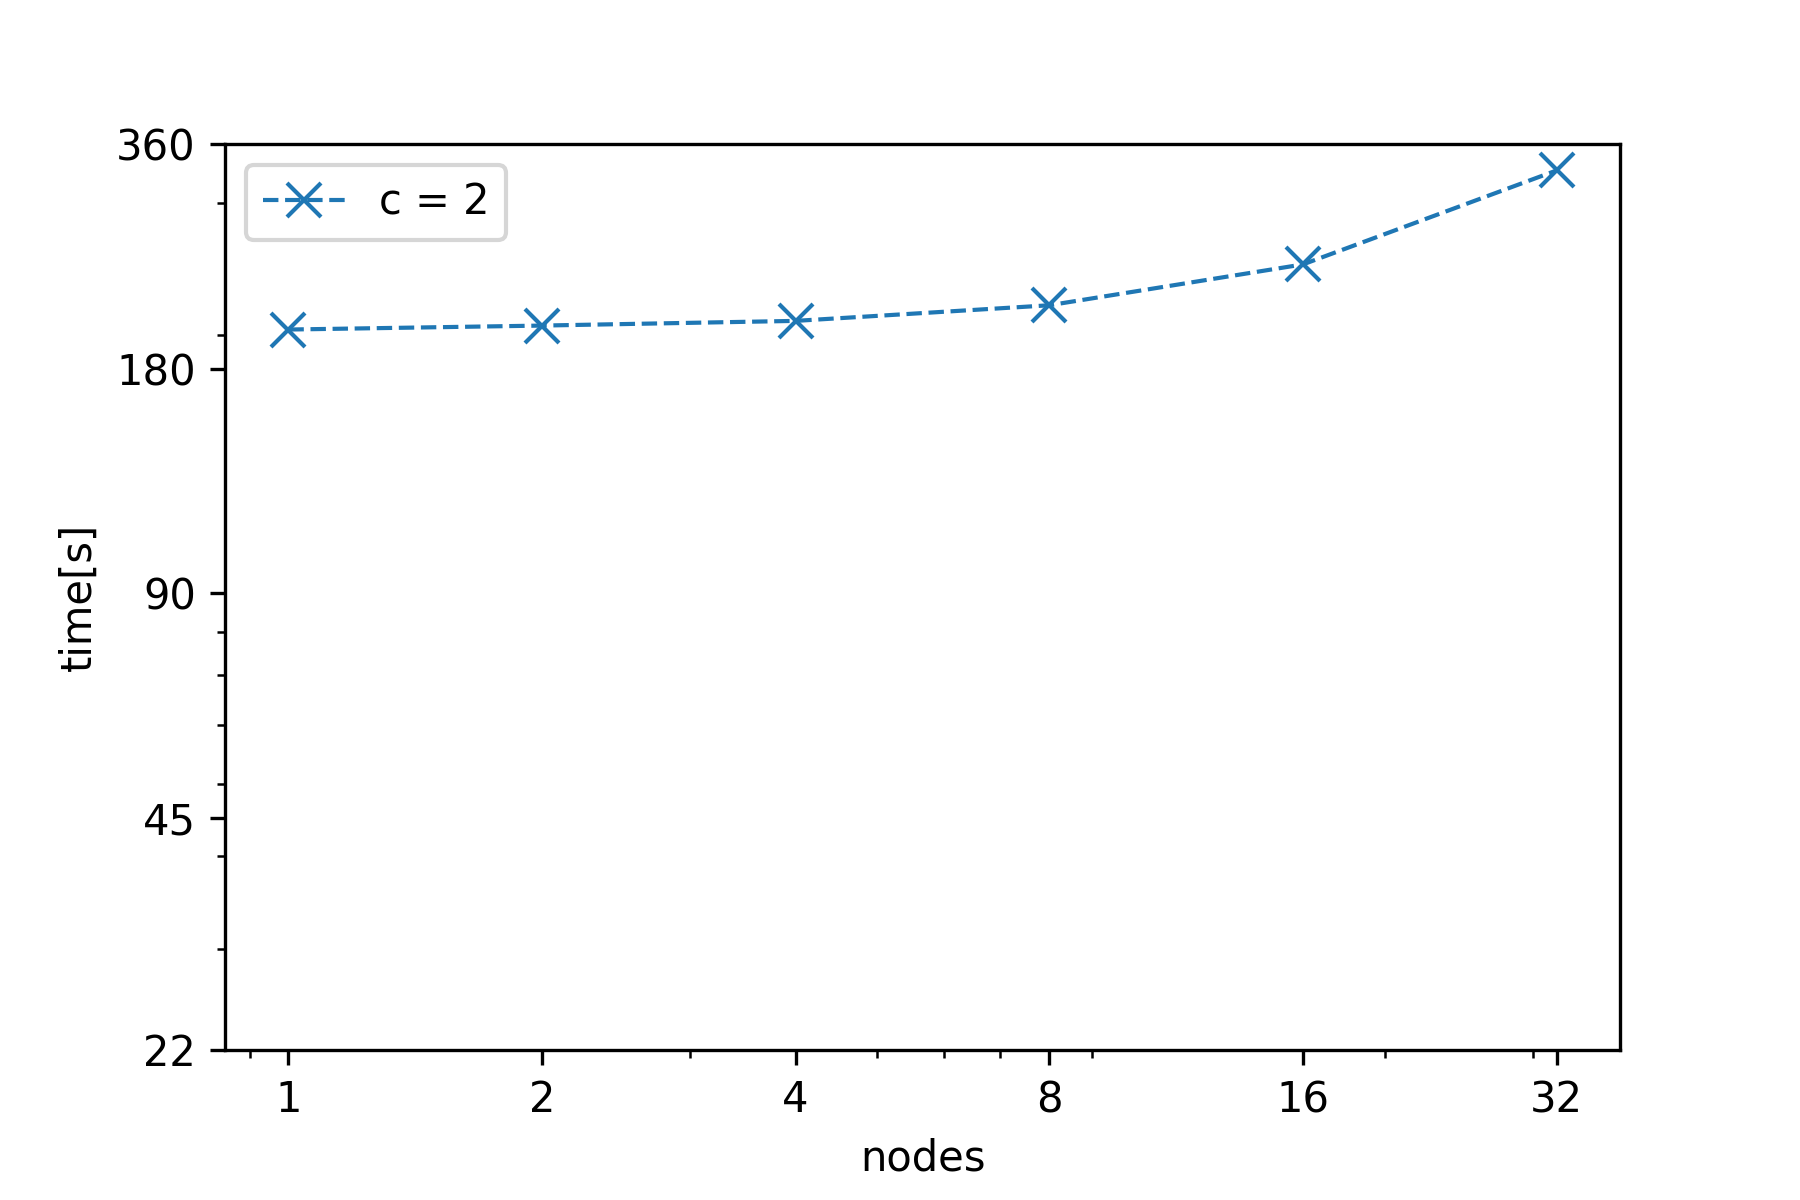
\includegraphics[width=\textwidth]{charts/s_50000_1000_weak_i_m}
        \caption{InnerABC, MKL}
    \end{subfigure}
    \caption{Słaba skalowalność. Czasy dla $n=50000, d=1000, e=nodes \times 5, \text{tasks-per-node}=24$}\label{fig:animals}
    \label{fig:scal_weak}
\end{figure}


\end{document}